%--------------------------------------
%ELECTROTECHNIQUE - SCHEMA DE LIAISON A LA TERRE
%--------------------------------------

%utiliser les environnement \begin{comment} \end{comment} pour mettre en commentaire le préambule une fois la programmation appelée dans le document maître (!ne pas oublier de mettre en commentaire \end{document}!)

%\begin{comment}

\documentclass[a4paper, 11pt, twoside, fleqn]{memoir}

\usepackage{AOCDTF}

\marqueurchapitre

%--------------------------------------
%corps du document
%--------------------------------------

\begin{document} %corps du document
	\openleft %début de chapitre à gauche

%\end{comment}

\chapter{Schéma Terre-Neutre}
\ChapFrame

\section{Caractéristiques générales}

\begin{definition}[Schéma TN]
Schéma de liaison à la terre dans lequel :
\begin{description}
\item[Neutre :] relié à la terre\,;
\item[Masse :] reliées au neutre du transformateur HT/BT.
\end{description}
\end{definition}

Dans le SLT TN, le point neutre du transformateur HT/BT (point commun) est relié à la terre via la \emph{prise de terre du neutre} \Circled{1}. Cette liaison présente une certaine résistance, la \emph{résistance de la prise de terre du neutre} $R_B$ \Circled{2}. Sa mise en \oe{}uvre est à charge du fournisseur d'électricité et sa résistance globale doit être inférieure ou égale à \SI{15}{\ohm} \supercite{NF:C13-100-2015}.\\
Les masses sont quant à elles reliées au point neutre du transformateur HT/BT (point commun), cela est réalisé via trois déclinaisons du SLT différentes :

\begin{description}
\item{TN-C :} le conducteur neutre et PE sont Confondus, le conducteur neutre devient donc vert/jaune et s'appelle dès lors conducteur Protection \'Equipotentielle Neutre (PEN).
\item{TN-S :} le conducteur neutre et PE sont Séparés, le conducteur neutre et le conducteur PE (PE+N) sont connectés dans le poste HT/BT.
\item{TN-C-S :} le conducteur neutre et PE sont Séparés et Confondus sur une même installation, le SLT TN-C ne devant jamais être utilisé en aval du SLT TN-S.
\end{description}
\section{Schémas de principe}

\begin{figure}[h]
\caption{Installation Terre-Neutre Confondu}
\begin{subfigure}[t]{0.49\linewidth}
\input{fig_schema_tn_sain}
\subcaption{sans défaut d'isolement}
\end{subfigure}
\begin{subfigure}[t]{0.49\linewidth}
%--------------------------------------
%ELECTROTECHNIQUE - SCHEMA DE LIAISON A LA TERRE
%--------------------------------------

%utiliser les environnement \begin{comment} \end{comment} pour mettre en commentaire le préambule une fois la programmation appelée dans le document maître (!ne pas oublier de mettre en commentaire \end{document}!)

\begin{comment}

\documentclass[a4paper, 11pt, twoside, fleqn]{memoir}

\usepackage{AOCDTF}

\marqueurchapitre

%lien d'édition des figures Tikz sur le site mathcha.io (rajouter le lien d'une modification effectuée sur la figure tikz avec le nom du modificateur car il n'y a qu'un lien par compte)

%lien mathcha Bruno Douchy : https://www.mathcha.io/editor/eKlmwIEXSj3Czgp1ZlU5eo1ZqI4VwNeYHpB7zQK

%--------------------------------------
%corps du document
%--------------------------------------

\begin{document} %corps du document
	\openleft %début de chapitre à gauche

\end{comment}





% Pattern Info
 
\tikzset{
pattern size/.store in=\mcSize, 
pattern size = 5pt,
pattern thickness/.store in=\mcThickness, 
pattern thickness = 0.3pt,
pattern radius/.store in=\mcRadius, 
pattern radius = 1pt}
\makeatletter
\pgfutil@ifundefined{pgf@pattern@name@_ma9nw6vc8}{
\pgfdeclarepatternformonly[\mcThickness,\mcSize]{_ma9nw6vc8}
{\pgfqpoint{0pt}{0pt}}
{\pgfpoint{\mcSize+\mcThickness}{\mcSize+\mcThickness}}
{\pgfpoint{\mcSize}{\mcSize}}
{
\pgfsetcolor{\tikz@pattern@color}
\pgfsetlinewidth{\mcThickness}
\pgfpathmoveto{\pgfqpoint{0pt}{0pt}}
\pgfpathlineto{\pgfpoint{\mcSize+\mcThickness}{\mcSize+\mcThickness}}
\pgfusepath{stroke}
}}
\makeatother
\tikzset{every picture/.style={line width=0.5pt}} %set default line width to 0.75pt        

\begin{tikzpicture}[x=0.75pt,y=0.75pt,yscale=-0.6,xscale=0.6]
%uncomment if require: \path (0,293); %set diagram left start at 0, and has height of 293

%Straight Lines [id:da8171558078184873] 
\draw [color={rgb, 255:red, 248; green, 231; blue, 28 }  ,draw opacity=1 ]   (90,75) -- (460,75) ;
%Straight Lines [id:da16438907305411632] 
\draw [color={rgb, 255:red, 126; green, 211; blue, 33 }  ,draw opacity=1 ] [dash pattern={on 4.5pt off 4.5pt}]  (90,75) -- (460,75) ;
%Straight Lines [id:da3591349784222725] 
\draw [color={rgb, 255:red, 248; green, 231; blue, 28 }  ,draw opacity=1 ]   (87.5,222.5) -- (87.5,252.5) ;
%Straight Lines [id:da008765067779469726] 
\draw [color={rgb, 255:red, 248; green, 231; blue, 28 }  ,draw opacity=1 ]   (240,135) -- (225,135) -- (225,75) ;
%Straight Lines [id:da9996152121194258] 
\draw    (120,35) -- (162.5,35) ;
%Straight Lines [id:da5023751395172481] 
\draw [color={rgb, 255:red, 139; green, 87; blue, 42 }  ,draw opacity=1 ]   (112.5,15) -- (162.5,15) ;
%Straight Lines [id:da6629450629275421] 
\draw [color={rgb, 255:red, 155; green, 155; blue, 155 }  ,draw opacity=1 ]   (112.5,55) -- (162.5,55) ;
%Straight Lines [id:da7406348808045065] 
\draw [color={rgb, 255:red, 248; green, 231; blue, 28 }  ,draw opacity=1 ]   (95.5,35) -- (87.5,75) -- (87.5,182.5) ;
%Straight Lines [id:da8967520631020585] 
\draw [color={rgb, 255:red, 126; green, 211; blue, 33 }  ,draw opacity=1 ] [dash pattern={on 4.5pt off 4.5pt}]  (95.5,35) -- (87.5,75) -- (87.5,182.5) ;
%Shape: Circle [id:dp0027818785253741485] 
\draw  [fill={rgb, 255:red, 0; green, 0; blue, 0 }  ,fill opacity=1 ] (85,75) .. controls (85,73.62) and (86.12,72.5) .. (87.5,72.5) .. controls (88.88,72.5) and (90,73.62) .. (90,75) .. controls (90,76.38) and (88.88,77.5) .. (87.5,77.5) .. controls (86.12,77.5) and (85,76.38) .. (85,75) -- cycle ;
%Straight Lines [id:da5752741404016657] 
\draw    (202.5,35) -- (460,35) ;
%Straight Lines [id:da4814004273751151] 
\draw [color={rgb, 255:red, 139; green, 87; blue, 42 }  ,draw opacity=1 ]   (202.5,15) -- (460,15) ;
%Straight Lines [id:da3315148063986225] 
\draw [color={rgb, 255:red, 155; green, 155; blue, 155 }  ,draw opacity=1 ]   (202.5,55) -- (460,55) ;
%Shape: Path Data [id:dp897526939895229] 
\draw   (112.5,55) .. controls (112.5,56.38) and (111.38,57.5) .. (110,57.5) .. controls (109.29,57.5) and (108.65,57.2) .. (108.19,56.72) .. controls (102.81,61.85) and (95.52,65) .. (87.5,65) .. controls (70.93,65) and (57.5,51.57) .. (57.5,35) .. controls (57.5,18.43) and (70.93,5) .. (87.5,5) .. controls (95.52,5) and (102.81,8.15) .. (108.19,13.28) .. controls (108.65,12.8) and (109.29,12.5) .. (110,12.5) .. controls (111.38,12.5) and (112.5,13.62) .. (112.5,15) .. controls (112.5,15.82) and (112.11,16.54) .. (111.5,17) .. controls (114.8,21.39) and (116.92,26.71) .. (117.4,32.5) .. controls (117.43,32.5) and (117.47,32.5) .. (117.5,32.5) .. controls (118.88,32.5) and (120,33.62) .. (120,35) .. controls (120,36.38) and (118.88,37.5) .. (117.5,37.5) .. controls (117.47,37.5) and (117.43,37.5) .. (117.4,37.5) .. controls (116.92,43.29) and (114.8,48.61) .. (111.5,53) .. controls (112.11,53.46) and (112.5,54.18) .. (112.5,55) -- cycle ;
%Shape: Circle [id:dp4775748559447114] 
\draw   (17.5,35) .. controls (17.5,18.43) and (30.93,5) .. (47.5,5) .. controls (64.07,5) and (77.5,18.43) .. (77.5,35) .. controls (77.5,51.57) and (64.07,65) .. (47.5,65) .. controls (30.93,65) and (17.5,51.57) .. (17.5,35) -- cycle ;
%Shape: Triangle [id:dp2038337174354391] 
\draw   (40,25) -- (30,42.5) -- (50,42.5) -- cycle ;
%Shape: Star [id:dp8001348775779505] 
\draw   (106.75,35) -- (95.5,35) -- (89.88,44.81) -- (95.5,35) -- (89.88,25.19) -- (95.5,35) -- cycle ;
%Shape: Circle [id:dp6579346258034324] 
\draw   (107.5,15) .. controls (107.5,13.62) and (108.62,12.5) .. (110,12.5) .. controls (111.38,12.5) and (112.5,13.62) .. (112.5,15) .. controls (112.5,16.38) and (111.38,17.5) .. (110,17.5) .. controls (108.62,17.5) and (107.5,16.38) .. (107.5,15) -- cycle ;
%Shape: Circle [id:dp8801072903263871] 
\draw   (114.9,35) .. controls (114.9,33.62) and (116.02,32.5) .. (117.4,32.5) .. controls (118.78,32.5) and (119.9,33.62) .. (119.9,35) .. controls (119.9,36.38) and (118.78,37.5) .. (117.4,37.5) .. controls (116.02,37.5) and (114.9,36.38) .. (114.9,35) -- cycle ;
%Shape: Circle [id:dp14922972530582124] 
\draw   (107.5,55) .. controls (107.5,53.62) and (108.62,52.5) .. (110,52.5) .. controls (111.38,52.5) and (112.5,53.62) .. (112.5,55) .. controls (112.5,56.38) and (111.38,57.5) .. (110,57.5) .. controls (108.62,57.5) and (107.5,56.38) .. (107.5,55) -- cycle ;

%Straight Lines [id:da20500240913471945] 
\draw [color={rgb, 255:red, 74; green, 144; blue, 226 }  ,draw opacity=1 ]   (292.5,112.5) -- (292.5,77.5) ;
%Straight Lines [id:da6309627145662347] 
\draw [color={rgb, 255:red, 139; green, 87; blue, 42 }  ,draw opacity=1 ]   (252.5,112.5) -- (252.5,17.5) ;
%Straight Lines [id:da3008435573206578] 
\draw [color={rgb, 255:red, 139; green, 87; blue, 42 }  ,draw opacity=1 ]   (252.5,130) -- (252.5,117.5) ;
%Straight Lines [id:da7919462422511667] 
\draw [color={rgb, 255:red, 74; green, 144; blue, 226 }  ,draw opacity=1 ]   (292.5,130.5) -- (292.5,117.5) ;
%Straight Lines [id:da07513748885898741] 
\draw    (45,230) -- (460,230) ;
%Shape: Rectangle [id:dp742088017567381] 
\draw  [draw opacity=0][pattern=_ma9nw6vc8,pattern size=6pt,pattern thickness=0.75pt,pattern radius=0pt, pattern color={rgb, 255:red, 0; green, 0; blue, 0}][line width=0.75]  (45,230) -- (460,230) -- (460,245) -- (45,245) -- cycle ;
%Straight Lines [id:da6254430679392561] 
\draw [color={rgb, 255:red, 126; green, 211; blue, 33 }  ,draw opacity=1 ] [dash pattern={on 4.5pt off 4.5pt}]  (240,135) -- (225,135) -- (225,75) ;
%Straight Lines [id:da6710590112346708] 
\draw    (87.5,252.5) -- (87.5,267.5) ;
%Straight Lines [id:da059383127594300866] 
\draw    (77.5,267.5) -- (97.5,267.5) ;
%Straight Lines [id:da5625728317663862] 
\draw    (80,272.5) -- (95,272.5) ;
%Straight Lines [id:da7240449748436714] 
\draw    (82.5,277.5) -- (92.5,277.5) ;

%Straight Lines [id:da247576449650577] 
\draw [color={rgb, 255:red, 126; green, 211; blue, 33 }  ,draw opacity=1 ] [dash pattern={on 4.5pt off 4.5pt}]  (87.5,222.5) -- (87.5,252.5) ;
%Straight Lines [id:da4314547900468141] 
\draw    (287.5,130) -- (292.5,130) ;
%Shape: Rectangle [id:dp693815005111987] 
\draw   (257.5,125) -- (287.5,125) -- (287.5,135) -- (257.5,135) -- cycle ;
%Straight Lines [id:da32763264490499355] 
\draw    (252.5,130) -- (257.5,130) ;

%Straight Lines [id:da15771842366117905] 
\draw    (87.5,217.5) -- (87.5,222.5) ;
%Shape: Rectangle [id:dp781974077045083] 
\draw   (92.5,187.5) -- (92.5,217.5) -- (82.5,217.5) -- (82.5,187.5) -- cycle ;
%Straight Lines [id:da2228121355456678] 
\draw    (87.5,182.5) -- (87.5,187.5) ;

%Straight Lines [id:da44489674368646215] 
\draw [color={rgb, 255:red, 248; green, 231; blue, 28 }  ,draw opacity=1 ]   (325,135) -- (310,135) -- (310,75) ;
%Straight Lines [id:da38264899651135764] 
\draw [color={rgb, 255:red, 74; green, 144; blue, 226 }  ,draw opacity=1 ]   (377.5,112.5) -- (377.5,77.5) ;
%Straight Lines [id:da5618192128083233] 
\draw [color={rgb, 255:red, 139; green, 87; blue, 42 }  ,draw opacity=1 ]   (337.5,112.5) -- (337.5,17.5) ;
%Straight Lines [id:da8381795635329556] 
\draw [color={rgb, 255:red, 139; green, 87; blue, 42 }  ,draw opacity=1 ]   (337.5,130) -- (337.5,117.5) ;
%Straight Lines [id:da1699886501918394] 
\draw [color={rgb, 255:red, 74; green, 144; blue, 226 }  ,draw opacity=1 ]   (377.5,130.5) -- (377.5,117.5) ;
%Straight Lines [id:da40404309478931644] 
\draw [color={rgb, 255:red, 126; green, 211; blue, 33 }  ,draw opacity=1 ] [dash pattern={on 4.5pt off 4.5pt}]  (325,135) -- (310,135) -- (310,75) ;
%Straight Lines [id:da17382635237392474] 
\draw    (372.5,130) -- (377.5,130) ;
%Shape: Rectangle [id:dp5713440724970389] 
\draw   (342.5,125) -- (372.5,125) -- (372.5,135) -- (342.5,135) -- cycle ;
%Straight Lines [id:da6072565548409633] 
\draw    (337.5,130) -- (342.5,130) ;

%Straight Lines [id:da46432540653799903] 
\draw [color={rgb, 255:red, 248; green, 231; blue, 28 }  ,draw opacity=1 ]   (410,135) -- (395,135) -- (395,75) ;
%Straight Lines [id:da555116694872677] 
\draw [color={rgb, 255:red, 74; green, 144; blue, 226 }  ,draw opacity=1 ]   (462.5,112.5) -- (462.5,77.5) ;
%Straight Lines [id:da6107719824468321] 
\draw [color={rgb, 255:red, 139; green, 87; blue, 42 }  ,draw opacity=1 ]   (422.5,112.5) -- (422.5,17.5) ;
%Straight Lines [id:da038679886271356434] 
\draw [color={rgb, 255:red, 139; green, 87; blue, 42 }  ,draw opacity=1 ]   (422.5,130) -- (422.5,117.5) ;
%Straight Lines [id:da7095727908104696] 
\draw [color={rgb, 255:red, 74; green, 144; blue, 226 }  ,draw opacity=1 ]   (462.5,130.5) -- (462.5,117.5) ;
%Straight Lines [id:da14055998525174573] 
\draw [color={rgb, 255:red, 126; green, 211; blue, 33 }  ,draw opacity=1 ] [dash pattern={on 4.5pt off 4.5pt}]  (412.5,135) -- (395,135) -- (395,75) ;
%Straight Lines [id:da9541765570709573] 
\draw    (457.5,130) -- (462.5,130) ;
%Shape: Rectangle [id:dp8186345814093839] 
\draw   (427.5,125) -- (457.5,125) -- (457.5,135) -- (427.5,135) -- cycle ;
%Straight Lines [id:da3329865721534958] 
\draw    (422.5,130) -- (427.5,130) ;

%Shape: Circle [id:dp4220828139965942] 
\draw  [fill={rgb, 255:red, 0; green, 0; blue, 0 }  ,fill opacity=1 ] (375,75) .. controls (375,73.62) and (376.12,72.5) .. (377.5,72.5) .. controls (378.88,72.5) and (380,73.62) .. (380,75) .. controls (380,76.38) and (378.88,77.5) .. (377.5,77.5) .. controls (376.12,77.5) and (375,76.38) .. (375,75) -- cycle ;
%Shape: Circle [id:dp27245203714964084] 
\draw  [fill={rgb, 255:red, 0; green, 0; blue, 0 }  ,fill opacity=1 ] (460,75) .. controls (460,73.62) and (461.12,72.5) .. (462.5,72.5) .. controls (463.88,72.5) and (465,73.62) .. (465,75) .. controls (465,76.38) and (463.88,77.5) .. (462.5,77.5) .. controls (461.12,77.5) and (460,76.38) .. (460,75) -- cycle ;
%Shape: Circle [id:dp9823963022345154] 
\draw  [fill={rgb, 255:red, 0; green, 0; blue, 0 }  ,fill opacity=1 ] (335,15) .. controls (335,13.62) and (336.12,12.5) .. (337.5,12.5) .. controls (338.88,12.5) and (340,13.62) .. (340,15) .. controls (340,16.38) and (338.88,17.5) .. (337.5,17.5) .. controls (336.12,17.5) and (335,16.38) .. (335,15) -- cycle ;
%Shape: Circle [id:dp6504746988474035] 
\draw  [fill={rgb, 255:red, 0; green, 0; blue, 0 }  ,fill opacity=1 ] (420,15) .. controls (420,13.62) and (421.12,12.5) .. (422.5,12.5) .. controls (423.88,12.5) and (425,13.62) .. (425,15) .. controls (425,16.38) and (423.88,17.5) .. (422.5,17.5) .. controls (421.12,17.5) and (420,16.38) .. (420,15) -- cycle ;
%Shape: Circle [id:dp853016740701949] 
\draw  [fill={rgb, 255:red, 0; green, 0; blue, 0 }  ,fill opacity=1 ] (290,75) .. controls (290,73.62) and (291.12,72.5) .. (292.5,72.5) .. controls (293.88,72.5) and (295,73.62) .. (295,75) .. controls (295,76.38) and (293.88,77.5) .. (292.5,77.5) .. controls (291.12,77.5) and (290,76.38) .. (290,75) -- cycle ;
%Shape: Circle [id:dp6925006431966902] 
\draw  [fill={rgb, 255:red, 0; green, 0; blue, 0 }  ,fill opacity=1 ] (250,15) .. controls (250,13.62) and (251.12,12.5) .. (252.5,12.5) .. controls (253.88,12.5) and (255,13.62) .. (255,15) .. controls (255,16.38) and (253.88,17.5) .. (252.5,17.5) .. controls (251.12,17.5) and (250,16.38) .. (250,15) -- cycle ;
%Shape: Rectangle [id:dp8918892221314038] 
\draw  [dash pattern={on 2.25pt off 2.25pt on 1pt off 2.25pt}] (242.5,115) -- (302.5,115) -- (302.5,145) -- (242.5,145) -- cycle ;
%Shape: Circle [id:dp7896916811705718] 
\draw  [fill={rgb, 255:red, 255; green, 255; blue, 255 }  ,fill opacity=1 ] (240,135) .. controls (240,133.62) and (241.12,132.5) .. (242.5,132.5) .. controls (243.88,132.5) and (245,133.62) .. (245,135) .. controls (245,136.38) and (243.88,137.5) .. (242.5,137.5) .. controls (241.12,137.5) and (240,136.38) .. (240,135) -- cycle ;
%Shape: Circle [id:dp43512583817576833] 
\draw  [fill={rgb, 255:red, 255; green, 255; blue, 255 }  ,fill opacity=1 ] (250,115) .. controls (250,113.62) and (251.12,112.5) .. (252.5,112.5) .. controls (253.88,112.5) and (255,113.62) .. (255,115) .. controls (255,116.38) and (253.88,117.5) .. (252.5,117.5) .. controls (251.12,117.5) and (250,116.38) .. (250,115) -- cycle ;
%Shape: Circle [id:dp5651828724211149] 
\draw  [fill={rgb, 255:red, 255; green, 255; blue, 255 }  ,fill opacity=1 ] (290,115) .. controls (290,113.62) and (291.12,112.5) .. (292.5,112.5) .. controls (293.88,112.5) and (295,113.62) .. (295,115) .. controls (295,116.38) and (293.88,117.5) .. (292.5,117.5) .. controls (291.12,117.5) and (290,116.38) .. (290,115) -- cycle ;
%Shape: Rectangle [id:dp15724818528279294] 
\draw  [dash pattern={on 2.25pt off 2.25pt on 1pt off 2.25pt}] (327.5,115) -- (387.5,115) -- (387.5,145) -- (327.5,145) -- cycle ;
%Shape: Circle [id:dp8875155556074055] 
\draw  [fill={rgb, 255:red, 255; green, 255; blue, 255 }  ,fill opacity=1 ] (325,135) .. controls (325,133.62) and (326.12,132.5) .. (327.5,132.5) .. controls (328.88,132.5) and (330,133.62) .. (330,135) .. controls (330,136.38) and (328.88,137.5) .. (327.5,137.5) .. controls (326.12,137.5) and (325,136.38) .. (325,135) -- cycle ;
%Shape: Circle [id:dp6258067054564275] 
\draw  [fill={rgb, 255:red, 255; green, 255; blue, 255 }  ,fill opacity=1 ] (335,115) .. controls (335,113.62) and (336.12,112.5) .. (337.5,112.5) .. controls (338.88,112.5) and (340,113.62) .. (340,115) .. controls (340,116.38) and (338.88,117.5) .. (337.5,117.5) .. controls (336.12,117.5) and (335,116.38) .. (335,115) -- cycle ;
%Shape: Circle [id:dp6445808082543435] 
\draw  [fill={rgb, 255:red, 255; green, 255; blue, 255 }  ,fill opacity=1 ] (375,115) .. controls (375,113.62) and (376.12,112.5) .. (377.5,112.5) .. controls (378.88,112.5) and (380,113.62) .. (380,115) .. controls (380,116.38) and (378.88,117.5) .. (377.5,117.5) .. controls (376.12,117.5) and (375,116.38) .. (375,115) -- cycle ;
%Shape: Rectangle [id:dp4457632538903006] 
\draw  [dash pattern={on 2.25pt off 2.25pt on 1pt off 2.25pt}] (412.5,115) -- (472.5,115) -- (472.5,145) -- (412.5,145) -- cycle ;
%Shape: Circle [id:dp0239014397171311] 
\draw  [fill={rgb, 255:red, 255; green, 255; blue, 255 }  ,fill opacity=1 ] (410,135) .. controls (410,133.62) and (411.12,132.5) .. (412.5,132.5) .. controls (413.88,132.5) and (415,133.62) .. (415,135) .. controls (415,136.38) and (413.88,137.5) .. (412.5,137.5) .. controls (411.12,137.5) and (410,136.38) .. (410,135) -- cycle ;
%Shape: Circle [id:dp8840214415867118] 
\draw  [fill={rgb, 255:red, 255; green, 255; blue, 255 }  ,fill opacity=1 ] (420,115) .. controls (420,113.62) and (421.12,112.5) .. (422.5,112.5) .. controls (423.88,112.5) and (425,113.62) .. (425,115) .. controls (425,116.38) and (423.88,117.5) .. (422.5,117.5) .. controls (421.12,117.5) and (420,116.38) .. (420,115) -- cycle ;
%Shape: Circle [id:dp6588211140174554] 
\draw  [fill={rgb, 255:red, 255; green, 255; blue, 255 }  ,fill opacity=1 ] (460,115) .. controls (460,113.62) and (461.12,112.5) .. (462.5,112.5) .. controls (463.88,112.5) and (465,113.62) .. (465,115) .. controls (465,116.38) and (463.88,117.5) .. (462.5,117.5) .. controls (461.12,117.5) and (460,116.38) .. (460,115) -- cycle ;
%Shape: Boxed Line [id:dp5097340580389993] 
\draw    (274.27,88.83) -- (258.39,101.97) -- (270.89,101.86) -- (257.31,113.09) ;
\draw [shift={(255,115)}, rotate = 320.40999999999997] [fill={rgb, 255:red, 0; green, 0; blue, 0 }  ][line width=0.08]  [draw opacity=0] (5.36,-2.57) -- (0,0) -- (5.36,2.57) -- cycle    ;
%Shape: Circle [id:dp050991579611760596] 
\draw  [fill={rgb, 255:red, 0; green, 0; blue, 0 }  ,fill opacity=1 ] (307.5,75) .. controls (307.5,73.62) and (308.62,72.5) .. (310,72.5) .. controls (311.38,72.5) and (312.5,73.62) .. (312.5,75) .. controls (312.5,76.38) and (311.38,77.5) .. (310,77.5) .. controls (308.62,77.5) and (307.5,76.38) .. (307.5,75) -- cycle ;
%Shape: Circle [id:dp6739752990977529] 
\draw  [fill={rgb, 255:red, 0; green, 0; blue, 0 }  ,fill opacity=1 ] (392.5,75) .. controls (392.5,73.62) and (393.62,72.5) .. (395,72.5) .. controls (396.38,72.5) and (397.5,73.62) .. (397.5,75) .. controls (397.5,76.38) and (396.38,77.5) .. (395,77.5) .. controls (393.62,77.5) and (392.5,76.38) .. (392.5,75) -- cycle ;
%Shape: Circle [id:dp8032954955293198] 
\draw  [fill={rgb, 255:red, 0; green, 0; blue, 0 }  ,fill opacity=1 ] (222.5,75) .. controls (222.5,73.62) and (223.62,72.5) .. (225,72.5) .. controls (226.38,72.5) and (227.5,73.62) .. (227.5,75) .. controls (227.5,76.38) and (226.38,77.5) .. (225,77.5) .. controls (223.62,77.5) and (222.5,76.38) .. (222.5,75) -- cycle ;
%Straight Lines [id:da7042567897719704] 
\draw [color={rgb, 255:red, 208; green, 2; blue, 27 }  ,draw opacity=1 ] [dash pattern={on 0.75pt off 0.75pt}]  (110,15) .. controls (111.67,13.33) and (113.33,13.33) .. (115,15) .. controls (116.67,16.67) and (118.33,16.67) .. (120,15) .. controls (121.67,13.33) and (123.33,13.33) .. (125,15) .. controls (126.67,16.67) and (128.33,16.67) .. (130,15) .. controls (131.67,13.33) and (133.33,13.33) .. (135,15) .. controls (136.67,16.67) and (138.33,16.67) .. (140,15) .. controls (141.67,13.33) and (143.33,13.33) .. (145,15) .. controls (146.67,16.67) and (148.33,16.67) .. (150,15) .. controls (151.67,13.33) and (153.33,13.33) .. (155,15) .. controls (156.67,16.67) and (158.33,16.67) .. (160,15) .. controls (161.67,13.33) and (163.33,13.33) .. (165,15) .. controls (166.67,16.67) and (168.33,16.67) .. (170,15) .. controls (171.67,13.33) and (173.33,13.33) .. (175,15) .. controls (176.67,16.67) and (178.33,16.67) .. (180,15) .. controls (181.67,13.33) and (183.33,13.33) .. (185,15) .. controls (186.67,16.67) and (188.33,16.67) .. (190,15) .. controls (191.67,13.33) and (193.33,13.33) .. (195,15) .. controls (196.67,16.67) and (198.33,16.67) .. (200,15) .. controls (201.67,13.33) and (203.33,13.33) .. (205,15) .. controls (206.67,16.67) and (208.33,16.67) .. (210,15) .. controls (211.67,13.33) and (213.33,13.33) .. (215,15) .. controls (216.67,16.67) and (218.33,16.67) .. (220,15) .. controls (221.67,13.33) and (223.33,13.33) .. (225,15) .. controls (226.67,16.67) and (228.33,16.67) .. (230,15) .. controls (231.67,13.33) and (233.33,13.33) .. (235,15) .. controls (236.67,16.67) and (238.33,16.67) .. (240,15) .. controls (241.67,13.33) and (243.33,13.33) .. (245,15) .. controls (246.67,16.67) and (248.33,16.67) .. (250,15) -- (252.5,15) -- (252.5,15) .. controls (254.17,16.67) and (254.17,18.33) .. (252.5,20) .. controls (250.83,21.67) and (250.83,23.33) .. (252.5,25) .. controls (254.17,26.67) and (254.17,28.33) .. (252.5,30) .. controls (250.83,31.67) and (250.83,33.33) .. (252.5,35) .. controls (254.17,36.67) and (254.17,38.33) .. (252.5,40) .. controls (250.83,41.67) and (250.83,43.33) .. (252.5,45) .. controls (254.17,46.67) and (254.17,48.33) .. (252.5,50) .. controls (250.83,51.67) and (250.83,53.33) .. (252.5,55) .. controls (254.17,56.67) and (254.17,58.33) .. (252.5,60) .. controls (250.83,61.67) and (250.83,63.33) .. (252.5,65) .. controls (254.17,66.67) and (254.17,68.33) .. (252.5,70) .. controls (250.83,71.67) and (250.83,73.33) .. (252.5,75) .. controls (254.17,76.67) and (254.17,78.33) .. (252.5,80) .. controls (250.83,81.67) and (250.83,83.33) .. (252.5,85) .. controls (254.17,86.67) and (254.17,88.33) .. (252.5,90) .. controls (250.83,91.67) and (250.83,93.33) .. (252.5,95) .. controls (254.17,96.67) and (254.17,98.33) .. (252.5,100) .. controls (250.83,101.67) and (250.83,103.33) .. (252.5,105) .. controls (254.17,106.67) and (254.17,108.33) .. (252.5,110) -- (252.5,115) -- (252.5,115) .. controls (250.83,116.67) and (249.17,116.67) .. (247.5,115) .. controls (245.83,113.33) and (244.17,113.33) .. (242.5,115) -- (242.5,115) .. controls (244.17,116.67) and (244.17,118.33) .. (242.5,120) .. controls (240.83,121.67) and (240.83,123.33) .. (242.5,125) .. controls (244.17,126.67) and (244.17,128.33) .. (242.5,130) .. controls (240.83,131.67) and (240.83,133.33) .. (242.5,135) -- (242.5,135) -- (242.5,135) .. controls (240.83,136.67) and (239.17,136.67) .. (237.5,135) .. controls (235.83,133.33) and (234.17,133.33) .. (232.5,135) .. controls (230.83,136.67) and (229.17,136.67) .. (227.5,135) -- (225,135) -- (225,135) .. controls (223.33,133.33) and (223.33,131.67) .. (225,130) .. controls (226.67,128.33) and (226.67,126.67) .. (225,125) .. controls (223.33,123.33) and (223.33,121.67) .. (225,120) .. controls (226.67,118.33) and (226.67,116.67) .. (225,115) .. controls (223.33,113.33) and (223.33,111.67) .. (225,110) .. controls (226.67,108.33) and (226.67,106.67) .. (225,105) .. controls (223.33,103.33) and (223.33,101.67) .. (225,100) .. controls (226.67,98.33) and (226.67,96.67) .. (225,95) .. controls (223.33,93.33) and (223.33,91.67) .. (225,90) .. controls (226.67,88.33) and (226.67,86.67) .. (225,85) .. controls (223.33,83.33) and (223.33,81.67) .. (225,80) .. controls (226.67,78.33) and (226.67,76.67) .. (225,75) -- (225,75) -- (225,75) .. controls (223.33,76.67) and (221.67,76.67) .. (220,75) .. controls (218.33,73.33) and (216.67,73.33) .. (215,75) .. controls (213.33,76.67) and (211.67,76.67) .. (210,75) .. controls (208.33,73.33) and (206.67,73.33) .. (205,75) .. controls (203.33,76.67) and (201.67,76.67) .. (200,75) .. controls (198.33,73.33) and (196.67,73.33) .. (195,75) .. controls (193.33,76.67) and (191.67,76.67) .. (190,75) .. controls (188.33,73.33) and (186.67,73.33) .. (185,75) .. controls (183.33,76.67) and (181.67,76.67) .. (180,75) .. controls (178.33,73.33) and (176.67,73.33) .. (175,75) .. controls (173.33,76.67) and (171.67,76.67) .. (170,75) .. controls (168.33,73.33) and (166.67,73.33) .. (165,75) .. controls (163.33,76.67) and (161.67,76.67) .. (160,75) .. controls (158.33,73.33) and (156.67,73.33) .. (155,75) .. controls (153.33,76.67) and (151.67,76.67) .. (150,75) .. controls (148.33,73.33) and (146.67,73.33) .. (145,75) .. controls (143.33,76.67) and (141.67,76.67) .. (140,75) .. controls (138.33,73.33) and (136.67,73.33) .. (135,75) .. controls (133.33,76.67) and (131.67,76.67) .. (130,75) .. controls (128.33,73.33) and (126.67,73.33) .. (125,75) .. controls (123.33,76.67) and (121.67,76.67) .. (120,75) .. controls (118.33,73.33) and (116.67,73.33) .. (115,75) .. controls (113.33,76.67) and (111.67,76.67) .. (110,75) .. controls (108.33,73.33) and (106.67,73.33) .. (105,75) .. controls (103.33,76.67) and (101.67,76.67) .. (100,75) .. controls (98.33,73.33) and (96.67,73.33) .. (95,75) .. controls (93.33,76.67) and (91.67,76.67) .. (90,75) -- (87.5,75) -- (87.5,75) .. controls (86.19,73.04) and (86.52,71.41) .. (88.48,70.1) .. controls (90.44,68.79) and (90.77,67.15) .. (89.46,65.19) .. controls (88.15,63.23) and (88.48,61.6) .. (90.44,60.29) .. controls (92.4,58.98) and (92.73,57.35) .. (91.42,55.39) .. controls (90.11,53.43) and (90.44,51.8) .. (92.4,50.49) .. controls (94.36,49.18) and (94.69,47.54) .. (93.38,45.58) .. controls (92.07,43.62) and (92.4,41.99) .. (94.36,40.68) .. controls (96.32,39.37) and (96.65,37.74) .. (95.34,35.78) -- (95.5,35) -- (95.5,35) ;
%Straight Lines [id:da5923845750545604] 
\draw    (170.5,57) -- (192.5,55) -- (202.5,55) ;
%Straight Lines [id:da8618478445136096] 
\draw    (172.5,55) -- (162.5,55) ;
\draw [shift={(172.5,55)}, rotate = 225] [color={rgb, 255:red, 0; green, 0; blue, 0 }  ][line width=0.75]    (-3.35,0) -- (3.35,0)(0,3.35) -- (0,-3.35)   ;
%Straight Lines [id:da2518275015169922] 
\draw    (170.5,37) -- (192.5,35) -- (202.5,35) ;
%Straight Lines [id:da917073492863887] 
\draw  [dash pattern={on 4.5pt off 4.5pt}]  (181.5,56) -- (181.5,16) ;
%Straight Lines [id:da09388453096129323] 
\draw    (170.5,17) -- (192.5,15) -- (202.5,15) ;
%Straight Lines [id:da1547603434551973] 
\draw    (172.5,35) -- (162.5,35) ;
\draw [shift={(172.5,35)}, rotate = 225] [color={rgb, 255:red, 0; green, 0; blue, 0 }  ][line width=0.75]    (-3.35,0) -- (3.35,0)(0,3.35) -- (0,-3.35)   ;
%Straight Lines [id:da5852892895213968] 
\draw    (172.5,15) -- (162.5,15) ;
\draw [shift={(172.5,15)}, rotate = 225] [color={rgb, 255:red, 0; green, 0; blue, 0 }  ][line width=0.75]    (-3.35,0) -- (3.35,0)(0,3.35) -- (0,-3.35)   ;


% Text Node
\draw (94.5,190.5) node [anchor=north west][inner sep=0.75pt]   [align=left] {$R_b$};
% Text Node
\draw (294.5,93) node [anchor=north west][inner sep=0.75pt]   [align=left] {1};
% Text Node
\draw (379.5,93) node [anchor=north west][inner sep=0.75pt]   [align=left] {2};
% Text Node
\draw (464.5,93) node [anchor=north west][inner sep=0.75pt]   [align=left] {3};


\end{tikzpicture}


%\end{document}


\subcaption{avec défaut d'isolement}
\end{subfigure}
\end{figure}

En cas de défaut d'isolement sur les masses métalliques, le courant de défaut $I_d$ dispose d'un chemin, via le conducteur PEN, pour revenir au poste de transformateur HT/BT. Cela forme la \emph{boucle de défaut} qui s'apparente à un court-circuit.\\



Dans les calculs, il faut tenir compte de la \emph{résistance de défaut} $R_d$ qui prend en compte la nature du défaut d'isolement (franc ou non-franc) et la résistance de la carcasse métallique.\\

\pagebreak

%--------------------------------------
%ELECTROTECHNIQUE - SCHEMA DE LIAISON A LA TERRE
%--------------------------------------

%utiliser les environnement \begin{comment} \end{comment} pour mettre en commentaire le préambule une fois la programmation appelée dans le document maître (!ne pas oublier de mettre en commentaire \end{document}!)

\begin{comment}

\documentclass[a4paper, 11pt, twoside, fleqn]{memoir}

\usepackage{AOCDTF}

\marqueurchapitre

%lien de l'éditeur : https://www.mathcha.io/editor/W9VrNux1SnLu4o3Jm4hklNKwvuOwJ7XwCV6yqOW

%--------------------------------------
%corps du document
%--------------------------------------

\begin{document} %corps du document
	\openleft %début de chapitre à gauche

\end{comment}

\begin{figure}[H]
\caption{Boucle de défaut du courant $I_d$ sur L1}




\tikzset{every picture/.style={line width=0.75pt}} %set default line width to 0.75pt        

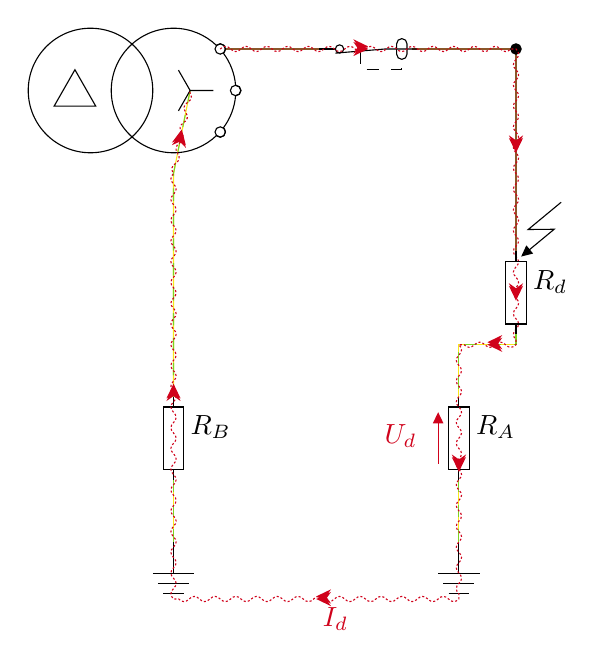
\begin{tikzpicture}[x=0.75pt,y=0.75pt,yscale=-1,xscale=1]
%uncomment if require: \path (0,353); %set diagram left start at 0, and has height of 353

%Straight Lines [id:da8450582290113836] 
\draw [color={rgb, 255:red, 248; green, 231; blue, 28 }  ,draw opacity=1 ]   (87.5,222.5) -- (87.5,252.5) ;
%Straight Lines [id:da035234150750507176] 
\draw [color={rgb, 255:red, 248; green, 231; blue, 28 }  ,draw opacity=1 ]   (252.5,152.5) -- (252.5,157.5) -- (225,157.5) -- (225,182.5) ;
%Straight Lines [id:da575921985906619] 
\draw [color={rgb, 255:red, 139; green, 87; blue, 42 }  ,draw opacity=1 ]   (112.5,15) -- (162.5,15) ;
%Straight Lines [id:da5726536295563455] 
\draw [color={rgb, 255:red, 248; green, 231; blue, 28 }  ,draw opacity=1 ]   (95.5,35) -- (87.5,75) -- (87.5,182.5) ;
%Straight Lines [id:da38476257001275427] 
\draw [color={rgb, 255:red, 126; green, 211; blue, 33 }  ,draw opacity=1 ] [dash pattern={on 4.5pt off 4.5pt}]  (95.5,35) -- (87.5,75) -- (87.5,182.5) ;
%Straight Lines [id:da9973940303994429] 
\draw [color={rgb, 255:red, 139; green, 87; blue, 42 }  ,draw opacity=1 ]   (202.5,15) -- (252.5,15) ;
%Shape: Path Data [id:dp9822778342813306] 
\draw   (112.5,55) .. controls (112.5,56.38) and (111.38,57.5) .. (110,57.5) .. controls (109.29,57.5) and (108.65,57.2) .. (108.19,56.72) .. controls (102.81,61.85) and (95.52,65) .. (87.5,65) .. controls (70.93,65) and (57.5,51.57) .. (57.5,35) .. controls (57.5,18.43) and (70.93,5) .. (87.5,5) .. controls (95.52,5) and (102.81,8.15) .. (108.19,13.28) .. controls (108.65,12.8) and (109.29,12.5) .. (110,12.5) .. controls (111.38,12.5) and (112.5,13.62) .. (112.5,15) .. controls (112.5,15.82) and (112.11,16.54) .. (111.5,17) .. controls (114.8,21.39) and (116.92,26.71) .. (117.4,32.5) .. controls (117.43,32.5) and (117.47,32.5) .. (117.5,32.5) .. controls (118.88,32.5) and (120,33.62) .. (120,35) .. controls (120,36.38) and (118.88,37.5) .. (117.5,37.5) .. controls (117.47,37.5) and (117.43,37.5) .. (117.4,37.5) .. controls (116.92,43.29) and (114.8,48.61) .. (111.5,53) .. controls (112.11,53.46) and (112.5,54.18) .. (112.5,55) -- cycle ;
%Shape: Circle [id:dp10169246549820965] 
\draw   (17.5,35) .. controls (17.5,18.43) and (30.93,5) .. (47.5,5) .. controls (64.07,5) and (77.5,18.43) .. (77.5,35) .. controls (77.5,51.57) and (64.07,65) .. (47.5,65) .. controls (30.93,65) and (17.5,51.57) .. (17.5,35) -- cycle ;
%Shape: Triangle [id:dp22185224755779764] 
\draw   (40,25) -- (30,42.5) -- (50,42.5) -- cycle ;
%Shape: Star [id:dp4535075510124722] 
\draw   (106.75,35) -- (95.5,35) -- (89.88,44.81) -- (95.5,35) -- (89.88,25.19) -- (95.5,35) -- cycle ;
%Shape: Circle [id:dp28187455970704567] 
\draw   (107.5,15) .. controls (107.5,13.62) and (108.62,12.5) .. (110,12.5) .. controls (111.38,12.5) and (112.5,13.62) .. (112.5,15) .. controls (112.5,16.38) and (111.38,17.5) .. (110,17.5) .. controls (108.62,17.5) and (107.5,16.38) .. (107.5,15) -- cycle ;
%Shape: Circle [id:dp9096244123377861] 
\draw   (114.9,35) .. controls (114.9,33.62) and (116.02,32.5) .. (117.4,32.5) .. controls (118.78,32.5) and (119.9,33.62) .. (119.9,35) .. controls (119.9,36.38) and (118.78,37.5) .. (117.4,37.5) .. controls (116.02,37.5) and (114.9,36.38) .. (114.9,35) -- cycle ;
%Shape: Circle [id:dp0660770114066822] 
\draw   (107.5,55) .. controls (107.5,53.62) and (108.62,52.5) .. (110,52.5) .. controls (111.38,52.5) and (112.5,53.62) .. (112.5,55) .. controls (112.5,56.38) and (111.38,57.5) .. (110,57.5) .. controls (108.62,57.5) and (107.5,56.38) .. (107.5,55) -- cycle ;

%Straight Lines [id:da12486709959480935] 
\draw [color={rgb, 255:red, 139; green, 87; blue, 42 }  ,draw opacity=1 ]   (252.5,112.5) -- (252.5,17.5) ;
%Straight Lines [id:da9194886303106931] 
\draw [color={rgb, 255:red, 126; green, 211; blue, 33 }  ,draw opacity=1 ] [dash pattern={on 4.5pt off 4.5pt}]  (252.5,152.5) -- (252.5,157.5) -- (225,157.5) -- (225,182.5) ;
%Straight Lines [id:da33889517147418446] 
\draw    (87.5,252.5) -- (87.5,267.5) ;
%Straight Lines [id:da7536356147270271] 
\draw    (77.5,267.5) -- (97.5,267.5) ;
%Straight Lines [id:da33790733335159795] 
\draw    (80,272.5) -- (95,272.5) ;
%Straight Lines [id:da8225336413065082] 
\draw    (82.5,277.5) -- (92.5,277.5) ;

%Straight Lines [id:da14728368722832463] 
\draw [color={rgb, 255:red, 126; green, 211; blue, 33 }  ,draw opacity=1 ] [dash pattern={on 4.5pt off 4.5pt}]  (87.5,222.5) -- (87.5,252.5) ;
%Straight Lines [id:da2713756434582886] 
\draw [color={rgb, 255:red, 248; green, 231; blue, 28 }  ,draw opacity=1 ]   (225,222.5) -- (225,252.5) ;
%Straight Lines [id:da07200185094723521] 
\draw    (225,252.5) -- (225,267.5) ;
%Straight Lines [id:da5503731135148442] 
\draw    (215,267.5) -- (235,267.5) ;
%Straight Lines [id:da9244125108161202] 
\draw    (217.5,272.5) -- (232.5,272.5) ;
%Straight Lines [id:da07512791048030887] 
\draw    (220,277.5) -- (230,277.5) ;

%Straight Lines [id:da5491926071123034] 
\draw [color={rgb, 255:red, 126; green, 211; blue, 33 }  ,draw opacity=1 ] [dash pattern={on 4.5pt off 4.5pt}]  (225,222.5) -- (225,252.5) ;
%Straight Lines [id:da7705666086878261] 
\draw    (87.5,217.5) -- (87.5,222.5) ;
%Shape: Rectangle [id:dp5724900932521552] 
\draw   (92.5,187.5) -- (92.5,217.5) -- (82.5,217.5) -- (82.5,187.5) -- cycle ;
%Straight Lines [id:da6857493814799358] 
\draw    (87.5,182.5) -- (87.5,187.5) ;

%Straight Lines [id:da7810225170823131] 
\draw    (225,217.5) -- (225,222.5) ;
%Shape: Rectangle [id:dp9839408028922504] 
\draw   (230,187.5) -- (230,217.5) -- (220,217.5) -- (220,187.5) -- cycle ;
%Straight Lines [id:da4367313473487816] 
\draw    (225,182.5) -- (225,187.5) ;

%Shape: Circle [id:dp6401617010113628] 
\draw  [fill={rgb, 255:red, 0; green, 0; blue, 0 }  ,fill opacity=1 ] (250,15) .. controls (250,13.62) and (251.12,12.5) .. (252.5,12.5) .. controls (253.88,12.5) and (255,13.62) .. (255,15) .. controls (255,16.38) and (253.88,17.5) .. (252.5,17.5) .. controls (251.12,17.5) and (250,16.38) .. (250,15) -- cycle ;
%Rounded Rect [id:dp9837999595449706] 
\draw   (197.5,20) .. controls (196.12,20) and (195,18.88) .. (195,17.5) -- (195,12.5) .. controls (195,11.12) and (196.12,10) .. (197.5,10) -- (197.5,10) .. controls (198.88,10) and (200,11.12) .. (200,12.5) -- (200,17.5) .. controls (200,18.88) and (198.88,20) .. (197.5,20) -- cycle ;
%Straight Lines [id:da04140906911364939] 
\draw  [dash pattern={on 4.5pt off 4.5pt}]  (177.5,16) -- (177.5,25) -- (197.5,25) -- (197.5,20) ;
%Shape: Circle [id:dp7012058816599942] 
\draw   (167.5,13) .. controls (166.4,13) and (165.5,13.9) .. (165.5,15) .. controls (165.5,16.1) and (166.4,17) .. (167.5,17) .. controls (168.6,17) and (169.5,16.1) .. (169.5,15) .. controls (169.5,13.9) and (168.6,13) .. (167.5,13) -- cycle ;
%Straight Lines [id:da23692932983683102] 
\draw    (165.5,15) -- (157.5,15) ;
%Straight Lines [id:da4567235518407359] 
\draw    (165.5,17) -- (189.5,15) -- (205,15) ;
%Shape: Boxed Line [id:dp44753967705251496] 
\draw    (274.27,88.83) -- (258.39,101.97) -- (270.89,101.86) -- (257.31,113.09) ;
\draw [shift={(255,115)}, rotate = 320.40999999999997] [fill={rgb, 255:red, 0; green, 0; blue, 0 }  ][line width=0.08]  [draw opacity=0] (5.36,-2.57) -- (0,0) -- (5.36,2.57) -- cycle    ;
\draw [color={rgb, 255:red, 208; green, 2; blue, 27 }  ,draw opacity=1 ] [dash pattern={on 0.75pt off 0.75pt}]  (110,15) .. controls (111.67,13.33) and (113.33,13.33) .. (115,15) .. controls (116.67,16.67) and (118.33,16.67) .. (120,15) .. controls (121.67,13.33) and (123.33,13.33) .. (125,15) .. controls (126.67,16.67) and (128.33,16.67) .. (130,15) .. controls (131.67,13.33) and (133.33,13.33) .. (135,15) .. controls (136.67,16.67) and (138.33,16.67) .. (140,15) .. controls (141.67,13.33) and (143.33,13.33) .. (145,15) .. controls (146.67,16.67) and (148.33,16.67) .. (150,15) .. controls (151.67,13.33) and (153.33,13.33) .. (155,15) .. controls (156.67,16.67) and (158.33,16.67) .. (160,15) .. controls (161.67,13.33) and (163.33,13.33) .. (165,15) .. controls (166.67,16.67) and (168.33,16.67) .. (170,15) .. controls (171.67,13.33) and (173.33,13.33) .. (175,15) .. controls (176.67,16.67) and (178.33,16.67) .. (180,15) .. controls (181.67,13.33) and (183.33,13.33) .. (185,15) .. controls (186.67,16.67) and (188.33,16.67) .. (190,15) .. controls (191.67,13.33) and (193.33,13.33) .. (195,15) .. controls (196.67,16.67) and (198.33,16.67) .. (200,15) .. controls (201.67,13.33) and (203.33,13.33) .. (205,15) .. controls (206.67,16.67) and (208.33,16.67) .. (210,15) .. controls (211.67,13.33) and (213.33,13.33) .. (215,15) .. controls (216.67,16.67) and (218.33,16.67) .. (220,15) .. controls (221.67,13.33) and (223.33,13.33) .. (225,15) .. controls (226.67,16.67) and (228.33,16.67) .. (230,15) .. controls (231.67,13.33) and (233.33,13.33) .. (235,15) .. controls (236.67,16.67) and (238.33,16.67) .. (240,15) .. controls (241.67,13.33) and (243.33,13.33) .. (245,15) .. controls (246.67,16.67) and (248.33,16.67) .. (250,15) -- (252.5,15) -- (252.5,15) .. controls (254.17,16.67) and (254.17,18.33) .. (252.5,20) .. controls (250.83,21.67) and (250.83,23.33) .. (252.5,25) .. controls (254.17,26.67) and (254.17,28.33) .. (252.5,30) .. controls (250.83,31.67) and (250.83,33.33) .. (252.5,35) .. controls (254.17,36.67) and (254.17,38.33) .. (252.5,40) .. controls (250.83,41.67) and (250.83,43.33) .. (252.5,45) .. controls (254.17,46.67) and (254.17,48.33) .. (252.5,50) .. controls (250.83,51.67) and (250.83,53.33) .. (252.5,55) .. controls (254.17,56.67) and (254.17,58.33) .. (252.5,60) .. controls (250.83,61.67) and (250.83,63.33) .. (252.5,65) .. controls (254.17,66.67) and (254.17,68.33) .. (252.5,70) .. controls (250.83,71.67) and (250.83,73.33) .. (252.5,75) .. controls (254.17,76.67) and (254.17,78.33) .. (252.5,80) .. controls (250.83,81.67) and (250.83,83.33) .. (252.5,85) .. controls (254.17,86.67) and (254.17,88.33) .. (252.5,90) .. controls (250.83,91.67) and (250.83,93.33) .. (252.5,95) .. controls (254.17,96.67) and (254.17,98.33) .. (252.5,100) .. controls (250.83,101.67) and (250.83,103.33) .. (252.5,105) .. controls (254.17,106.67) and (254.17,108.33) .. (252.5,110) .. controls (250.83,111.67) and (250.83,113.33) .. (252.5,115) -- (252.5,115) .. controls (254.17,116.67) and (254.17,118.33) .. (252.5,120) .. controls (250.83,121.67) and (250.83,123.33) .. (252.5,125) .. controls (254.17,126.67) and (254.17,128.33) .. (252.5,130) .. controls (250.83,131.67) and (250.83,133.33) .. (252.5,135) .. controls (254.17,136.67) and (254.17,138.33) .. (252.5,140) .. controls (250.83,141.67) and (250.83,143.33) .. (252.5,145) .. controls (254.17,146.67) and (254.17,148.33) .. (252.5,150) .. controls (250.83,151.67) and (250.83,153.33) .. (252.5,155) -- (252.5,157.5) -- (252.5,157.5) .. controls (250.83,159.17) and (249.17,159.17) .. (247.5,157.5) .. controls (245.83,155.83) and (244.17,155.83) .. (242.5,157.5) .. controls (240.83,159.17) and (239.17,159.17) .. (237.5,157.5) .. controls (235.83,155.83) and (234.17,155.83) .. (232.5,157.5) .. controls (230.83,159.17) and (229.17,159.17) .. (227.5,157.5) -- (225,157.5) -- (225,157.5) .. controls (226.67,159.17) and (226.67,160.83) .. (225,162.5) .. controls (223.33,164.17) and (223.33,165.83) .. (225,167.5) .. controls (226.67,169.17) and (226.67,170.83) .. (225,172.5) .. controls (223.33,174.17) and (223.33,175.83) .. (225,177.5) .. controls (226.67,179.17) and (226.67,180.83) .. (225,182.5) .. controls (223.33,184.17) and (223.33,185.83) .. (225,187.5) .. controls (226.67,189.17) and (226.67,190.83) .. (225,192.5) .. controls (223.33,194.17) and (223.33,195.83) .. (225,197.5) .. controls (226.67,199.17) and (226.67,200.83) .. (225,202.5) .. controls (223.33,204.17) and (223.33,205.83) .. (225,207.5) .. controls (226.67,209.17) and (226.67,210.83) .. (225,212.5) .. controls (223.33,214.17) and (223.33,215.83) .. (225,217.5) .. controls (226.67,219.17) and (226.67,220.83) .. (225,222.5) .. controls (223.33,224.17) and (223.33,225.83) .. (225,227.5) .. controls (226.67,229.17) and (226.67,230.83) .. (225,232.5) .. controls (223.33,234.17) and (223.33,235.83) .. (225,237.5) .. controls (226.67,239.17) and (226.67,240.83) .. (225,242.5) .. controls (223.33,244.17) and (223.33,245.83) .. (225,247.5) .. controls (226.67,249.17) and (226.67,250.83) .. (225,252.5) .. controls (223.33,254.17) and (223.33,255.83) .. (225,257.5) .. controls (226.67,259.17) and (226.67,260.83) .. (225,262.5) .. controls (223.33,264.17) and (223.33,265.83) .. (225,267.5) .. controls (226.67,269.17) and (226.67,270.83) .. (225,272.5) .. controls (223.33,274.17) and (223.33,275.83) .. (225,277.5) -- (225,280) -- (225,280) .. controls (223.33,281.67) and (221.67,281.67) .. (220,280) .. controls (218.33,278.33) and (216.67,278.33) .. (215,280) .. controls (213.33,281.67) and (211.67,281.67) .. (210,280) .. controls (208.33,278.33) and (206.67,278.33) .. (205,280) .. controls (203.33,281.67) and (201.67,281.67) .. (200,280) .. controls (198.33,278.33) and (196.67,278.33) .. (195,280) .. controls (193.33,281.67) and (191.67,281.67) .. (190,280) .. controls (188.33,278.33) and (186.67,278.33) .. (185,280) .. controls (183.33,281.67) and (181.67,281.67) .. (180,280) .. controls (178.33,278.33) and (176.67,278.33) .. (175,280) .. controls (173.33,281.67) and (171.67,281.67) .. (170,280) .. controls (168.33,278.33) and (166.67,278.33) .. (165,280) .. controls (163.33,281.67) and (161.67,281.67) .. (160,280) .. controls (158.33,278.33) and (156.67,278.33) .. (155,280) .. controls (153.33,281.67) and (151.67,281.67) .. (150,280) .. controls (148.33,278.33) and (146.67,278.33) .. (145,280) .. controls (143.33,281.67) and (141.67,281.67) .. (140,280) .. controls (138.33,278.33) and (136.67,278.33) .. (135,280) .. controls (133.33,281.67) and (131.67,281.67) .. (130,280) .. controls (128.33,278.33) and (126.67,278.33) .. (125,280) .. controls (123.33,281.67) and (121.67,281.67) .. (120,280) .. controls (118.33,278.33) and (116.67,278.33) .. (115,280) .. controls (113.33,281.67) and (111.67,281.67) .. (110,280) .. controls (108.33,278.33) and (106.67,278.33) .. (105,280) .. controls (103.33,281.67) and (101.67,281.67) .. (100,280) .. controls (98.33,278.33) and (96.67,278.33) .. (95,280) .. controls (93.33,281.67) and (91.67,281.67) .. (90,280) -- (87.5,280) -- (87.5,280) .. controls (85.83,278.33) and (85.83,276.67) .. (87.5,275) .. controls (89.17,273.33) and (89.17,271.67) .. (87.5,270) .. controls (85.83,268.33) and (85.83,266.67) .. (87.5,265) .. controls (89.17,263.33) and (89.17,261.67) .. (87.5,260) .. controls (85.83,258.33) and (85.83,256.67) .. (87.5,255) .. controls (89.17,253.33) and (89.17,251.67) .. (87.5,250) .. controls (85.83,248.33) and (85.83,246.67) .. (87.5,245) .. controls (89.17,243.33) and (89.17,241.67) .. (87.5,240) .. controls (85.83,238.33) and (85.83,236.67) .. (87.5,235) .. controls (89.17,233.33) and (89.17,231.67) .. (87.5,230) .. controls (85.83,228.33) and (85.83,226.67) .. (87.5,225) .. controls (89.17,223.33) and (89.17,221.67) .. (87.5,220) .. controls (85.83,218.33) and (85.83,216.67) .. (87.5,215) .. controls (89.17,213.33) and (89.17,211.67) .. (87.5,210) .. controls (85.83,208.33) and (85.83,206.67) .. (87.5,205) .. controls (89.17,203.33) and (89.17,201.67) .. (87.5,200) .. controls (85.83,198.33) and (85.83,196.67) .. (87.5,195) .. controls (89.17,193.33) and (89.17,191.67) .. (87.5,190) .. controls (85.83,188.33) and (85.83,186.67) .. (87.5,185) .. controls (89.17,183.33) and (89.17,181.67) .. (87.5,180) .. controls (85.83,178.33) and (85.83,176.67) .. (87.5,175) .. controls (89.17,173.33) and (89.17,171.67) .. (87.5,170) .. controls (85.83,168.33) and (85.83,166.67) .. (87.5,165) .. controls (89.17,163.33) and (89.17,161.67) .. (87.5,160) .. controls (85.83,158.33) and (85.83,156.67) .. (87.5,155) .. controls (89.17,153.33) and (89.17,151.67) .. (87.5,150) .. controls (85.83,148.33) and (85.83,146.67) .. (87.5,145) .. controls (89.17,143.33) and (89.17,141.67) .. (87.5,140) .. controls (85.83,138.33) and (85.83,136.67) .. (87.5,135) .. controls (89.17,133.33) and (89.17,131.67) .. (87.5,130) .. controls (85.83,128.33) and (85.83,126.67) .. (87.5,125) .. controls (89.17,123.33) and (89.17,121.67) .. (87.5,120) .. controls (85.83,118.33) and (85.83,116.67) .. (87.5,115) .. controls (89.17,113.33) and (89.17,111.67) .. (87.5,110) .. controls (85.83,108.33) and (85.83,106.67) .. (87.5,105) .. controls (89.17,103.33) and (89.17,101.67) .. (87.5,100) .. controls (85.83,98.33) and (85.83,96.67) .. (87.5,95) .. controls (89.17,93.33) and (89.17,91.67) .. (87.5,90) .. controls (85.83,88.33) and (85.83,86.67) .. (87.5,85) .. controls (89.17,83.33) and (89.17,81.67) .. (87.5,80) .. controls (85.83,78.33) and (85.83,76.67) .. (87.5,75) -- (87.5,75) .. controls (86.19,73.04) and (86.52,71.41) .. (88.48,70.1) .. controls (90.44,68.79) and (90.77,67.15) .. (89.46,65.19) .. controls (88.15,63.23) and (88.48,61.6) .. (90.44,60.29) .. controls (92.4,58.98) and (92.73,57.35) .. (91.42,55.39) .. controls (90.11,53.43) and (90.44,51.8) .. (92.4,50.49) .. controls (94.36,49.18) and (94.69,47.54) .. (93.38,45.58) .. controls (92.07,43.62) and (92.4,41.99) .. (94.36,40.68) .. controls (96.32,39.37) and (96.65,37.74) .. (95.34,35.78) -- (95.5,35) -- (95.5,35) ;
\draw [shift={(181.25,15)}, rotate = 180] [fill={rgb, 255:red, 208; green, 2; blue, 27 }  ,fill opacity=1 ][line width=0.08]  [draw opacity=0] (7.14,-3.43) -- (0,0) -- (7.14,3.43) -- (4.74,0) -- cycle    ;
\draw [shift={(252.5,65)}, rotate = 270] [fill={rgb, 255:red, 208; green, 2; blue, 27 }  ,fill opacity=1 ][line width=0.08]  [draw opacity=0] (7.14,-3.43) -- (0,0) -- (7.14,3.43) -- (4.74,0) -- cycle    ;
\draw [shift={(252.5,136.25)}, rotate = 270] [fill={rgb, 255:red, 208; green, 2; blue, 27 }  ,fill opacity=1 ][line width=0.08]  [draw opacity=0] (7.14,-3.43) -- (0,0) -- (7.14,3.43) -- (4.74,0) -- cycle    ;
\draw [shift={(238.75,157.5)}, rotate = 360] [fill={rgb, 255:red, 208; green, 2; blue, 27 }  ,fill opacity=1 ][line width=0.08]  [draw opacity=0] (7.14,-3.43) -- (0,0) -- (7.14,3.43) -- (4.74,0) -- cycle    ;
\draw [shift={(225,218.75)}, rotate = 270] [fill={rgb, 255:red, 208; green, 2; blue, 27 }  ,fill opacity=1 ][line width=0.08]  [draw opacity=0] (7.14,-3.43) -- (0,0) -- (7.14,3.43) -- (4.74,0) -- cycle    ;
\draw [shift={(156.25,280)}, rotate = 360] [fill={rgb, 255:red, 208; green, 2; blue, 27 }  ,fill opacity=1 ][line width=0.08]  [draw opacity=0] (7.14,-3.43) -- (0,0) -- (7.14,3.43) -- (4.74,0) -- cycle    ;
\draw [shift={(87.5,177.5)}, rotate = 450] [fill={rgb, 255:red, 208; green, 2; blue, 27 }  ,fill opacity=1 ][line width=0.08]  [draw opacity=0] (7.14,-3.43) -- (0,0) -- (7.14,3.43) -- (4.74,0) -- cycle    ;
\draw [shift={(91.5,55)}, rotate = 461.31] [fill={rgb, 255:red, 208; green, 2; blue, 27 }  ,fill opacity=1 ][line width=0.08]  [draw opacity=0] (7.14,-3.43) -- (0,0) -- (7.14,3.43) -- (4.74,0) -- cycle    ;
\draw [shift={(181.25,13.75)}, rotate = 180] [fill={rgb, 255:red, 208; green, 2; blue, 27 }  ,fill opacity=1 ][line width=0.08]  [draw opacity=0] (7.14,-3.43) -- (0,0) -- (7.14,3.43) -- (4.74,0) -- cycle    ;
\draw [shift={(252.5,63.75)}, rotate = 270] [fill={rgb, 255:red, 208; green, 2; blue, 27 }  ,fill opacity=1 ][line width=0.08]  [draw opacity=0] (7.14,-3.43) -- (0,0) -- (7.14,3.43) -- (4.74,0) -- cycle    ;
\draw [shift={(252.5,135)}, rotate = 270] [fill={rgb, 255:red, 208; green, 2; blue, 27 }  ,fill opacity=1 ][line width=0.08]  [draw opacity=0] (7.14,-3.43) -- (0,0) -- (7.14,3.43) -- (4.74,0) -- cycle    ;
\draw [shift={(238.75,156.25)}, rotate = 360] [fill={rgb, 255:red, 208; green, 2; blue, 27 }  ,fill opacity=1 ][line width=0.08]  [draw opacity=0] (7.14,-3.43) -- (0,0) -- (7.14,3.43) -- (4.74,0) -- cycle    ;
\draw [shift={(225,217.5)}, rotate = 270] [fill={rgb, 255:red, 208; green, 2; blue, 27 }  ,fill opacity=1 ][line width=0.08]  [draw opacity=0] (7.14,-3.43) -- (0,0) -- (7.14,3.43) -- (4.74,0) -- cycle    ;
\draw [shift={(156.25,278.75)}, rotate = 360] [fill={rgb, 255:red, 208; green, 2; blue, 27 }  ,fill opacity=1 ][line width=0.08]  [draw opacity=0] (7.14,-3.43) -- (0,0) -- (7.14,3.43) -- (4.74,0) -- cycle    ;
\draw [shift={(87.5,176.25)}, rotate = 450] [fill={rgb, 255:red, 208; green, 2; blue, 27 }  ,fill opacity=1 ][line width=0.08]  [draw opacity=0] (7.14,-3.43) -- (0,0) -- (7.14,3.43) -- (4.74,0) -- cycle    ;
\draw [shift={(91.5,53.75)}, rotate = 461.31] [fill={rgb, 255:red, 208; green, 2; blue, 27 }  ,fill opacity=1 ][line width=0.08]  [draw opacity=0] (7.14,-3.43) -- (0,0) -- (7.14,3.43) -- (4.74,0) -- cycle    ;
%Straight Lines [id:da9207949526828273] 
\draw    (252.5,147.5) -- (252.5,152.5) ;
%Shape: Rectangle [id:dp36210266951689685] 
\draw   (257.5,117.5) -- (257.5,147.5) -- (247.5,147.5) -- (247.5,117.5) -- cycle ;
%Straight Lines [id:da2843419817195654] 
\draw    (252.5,112.5) -- (252.5,117.5) ;

%Straight Lines [id:da667113945803525] 
\draw [color={rgb, 255:red, 208; green, 2; blue, 27 }  ,draw opacity=1 ]   (215,193) -- (215,215) ;
\draw [shift={(215,190)}, rotate = 90] [fill={rgb, 255:red, 208; green, 2; blue, 27 }  ,fill opacity=1 ][line width=0.08]  [draw opacity=0] (5.36,-2.57) -- (0,0) -- (5.36,2.57) -- cycle    ;

% Text Node
\draw (94.5,190.5) node [anchor=north west][inner sep=0.75pt]   [align=left] {$R_B$};
% Text Node
\draw (232,190.5) node [anchor=north west][inner sep=0.75pt]   [align=left] {$R_A$};
% Text Node
\draw (188,194.5) node [anchor=north west][inner sep=0.75pt]  [color={rgb, 255:red, 208; green, 2; blue, 27 }  ,opacity=1 ] [align=left] {$U_d$};
% Text Node
\draw (259.5,120.5) node [anchor=north west][inner sep=0.75pt]   [align=left] {$R_d$};
% Text Node
\draw (158.25,283) node [anchor=north west][inner sep=0.75pt] [color={rgb, 255:red, 208; green, 2; blue, 27 }]  [align=left] {$I_d$};


\end{tikzpicture}

\end{figure}

%\end{document}


\begin{comment}
\begin{circuitikz}[circuit ee IEC relay]
%\DrawGrid{(-1,-5)}{(9,3)} %grille d'aide pour le placement des objets

%alimentation

\node (D1) [make contact=point left, circuit breaker={point left}, tiny circuit symbols, activated] at (1,0.45) {};
\node (T1) [oosourcetransshape, prim=delta,sec=wye] at (0,0) {};


%neutre/terre

\node (RN) [R, label=$R_B$, rotate=90, tiny circuit symbols] at (0,-2.7) {};
\node (G1) [tlground] at (0,-3.9) {};
\draw [green!, thick] (G1) to node {} (RN) ; 
\draw [green!, thick] (RN) to (0,-0.5) to node {} (T1.sec4) ; 
\draw [dashed, yellow!, thick] (G1) to node {} (RN) ;
\draw [dashed, yellow!, thick] (RN) to (0,-0.5) to node {} (T1.sec4) ;

\node (RT) [resistor, rotate=90, tiny circuit symbols, label=$R_A$] at (2.5,-2.7) {};
\draw[-triangle 45, red] (2.8,-2) -- (2.8,-1) node[right,midway] {$U_d$};
\node (G2) [tlground] at (2.5,-3.9) {};
\draw [green!, thick] (RT) to (G2); 
\draw [dashed, yellow!, thick] (RT) to (G2);
\node (G2) [tlground] at (2.5,-3.9) {};
\draw [green!, thick] (G1) to (0,-4.2) to (2.5,-4.2) to (G2);
\draw [dashed, yellow!, thick] (G1) -- (0,-4.2) -- (2.5,-4.2) node [midway,below] {\color{black}$I_d$} -- (G2);
\node (G1) [tlground] at (0,-3.9) {};
\node (G2) [tlground] at (2.5,-3.9) {};

%appareil 1

\node (C2) [circ, scale=0.5] at (2.5,0.45) {};
\node (RD) [resistor, label=$R_d$, rotate=90, tiny circuit symbols] at (2.5,-1.5) {};

\draw [green!, thick] (RD) to (RT); 
\draw [dashed, yellow!, thick] (RD) to (RT); 

\draw [brown, thick] (T1.sec1) to (0.5,0.45) to (D1) to (C2) to (RD);
\node (T1) [oosourcetransshape, prim=delta,sec=wye] at (0,0) {};

%chemin courant

\fill [yellow!, decoration=lightning bolt, decorate] (2.5,-1.2) -- ++ (0.5,0.8); %éclairs
\path [postaction={on each segment={mid arrow=red}}]  (T1.sec1) -- (0.5,0.45) -- (D1) -- (C2) -- (RD) -- (RT) -- (G2) -- (2.5,-4.2) -- (1.666,-4.2) -- (0.88888,-4.2)  -- (0,-4.2) -- (G1) -- (RN) -- (0,-0.5) -- (T1.sec4); 

\callout{1,-0.5}{\cstep\label{pas:1}}{2.4,-1.2};


\end{circuitikz}
\end{comment}


L'intensité de courant $I_d$ vaut alors :
\begin{formule}[Courant de défaut $I_d$]
\begin{align}
		I_d &= \frac{V}{R_{B}+R_{A}+R_{d}}
\end{align}
\end{formule}

\begin{textvariables}
V								& tension							& volt			& \volt					& 	Différence de potentiel entre les masses métalliques et la terre 	\\
R_{B}						& résistance						& ohm			& \ohm					& 	Résistance de la prise de terre du neutre 	\\
R_{A}						& résistance						& ohm			& \ohm					& 	Résistance de la prise de terre de l'installation électrique 	\\
R_{d}						& résistance						& ohm			& \ohm					& 	Résistance de défaut 	d'isolement \\
\end{textvariables}

Le courant de défaut $I_d$ fera alors apparaître une \emph{tension de défaut} $U_d$ entre la masse métallique et la terre. Pour satisfaire aux normes de sécurité de la NF C15-100, il est imposé que la tension de défaut $U_d$ ne dépasse pas la tension de sécurité du local $U_L$ (voir \superref{subsec:prise_terre_installation_electrique}) :

\begin{formule}[Tension de défaut $U_d$]
\begin{align}
		U_d &= R_{A} \cdot I_{d} \\
			   &< U_L
\end{align}
\end{formule}

\begin{textvariables}
R_{A}						& résistance						& ohm			& \ohm					& 	Résistance de la prise de terre de l'installation électrique 	\\
I_{d}							& intensité							& ampère		& \ampere				& 	Courant de défaut d'isolement \\
U_{L}						& tension							& volt			& \volt					& 	Tension de sécurité du local avec :
\begin{description}[nosep, leftmargin=*]
\item[Local sec :] $U_{L}=\SI{50}{\volt}$
\item[Local humide :] $U_{L}=\SI{25}{\volt}$
\end{description} \\
\end{textvariables}

Il est donc nécessaire de limiter $U_d$ à la valeur suivante (voir \superref{form:resistance_prise_terre}) :

\begin{formule}[Calibre du DDR $I_{\Delta n}$]
\begin{align}
		I_{\Delta n} &< \frac{U_{L}}{R_{A}}
\end{align}
\end{formule}

\begin{textvariables}
U_{L}						& tension							& volt			& \volt					& 	Tension de sécurité du local avec :
\begin{description}[nosep, leftmargin=*]
\item[Local sec :] $U_{L}=\SI{50}{\volt}$
\item[Local humide :] $U_{L}=\SI{25}{\volt}$
\end{description} \\
R_{A}						& résistance						& ohm			& \ohm					& 	Résistance de la prise de terre de l'installation électrique 	\\
\end{textvariables}

\begin{exemple}[Calcul du calibre du DDR $I_{\Delta n}$]
Si on considère que le transformateur est un transformateur $\SI{20}{\kilo\volt}/\SI{400}{\volt}$, que $R_A=\SI{20}{\ohm}$, que $R_B=\SI{10}{\ohm}$ et que $R_d$ est négligée, on peut déduire que le courant de défaut $I_d$ vaut :
\begin{align*}
		I_d 	&= \frac{V}{R_{B}+R_{A}} \\
				&=\frac{400}{20+10} \\
				&= \SI{13,33}{\ampere} \\
\end{align*}
Si une personne touche une masse des récepteurs en défaut, elle sera soumise à une tension de défaut $U_d$ :
\begin{align*}
		U_d 	&= R_{A} \cdot I_{d} \\
				&=20 \cdot 13,33 \\
				&= \SI{266,6}{\volt}
\end{align*}
La tension de défaut $U_d$ est dangereuse quelle que soit la tension limite choisie :
\begin{itemize}
\item coupure la plus rapide possible\,;
\item protection des personnes.
\end{itemize}
~\\
\begin{minipage}[t]{0.5\linewidth}
Dans le cas d'un local sec :
\begin{align*}
	I_{\Delta n} 	&< \frac{U_{L}}{R_{A}} \\
						&< \frac{50}{20} \\
						&< \SI{2,5}{\ampere}
\end{align*}
\end{minipage}
\hfill
\begin{minipage}[t]{0.5\linewidth}
Dans le cas d'un local humide :
\begin{align*}
	I_{\Delta n} 	&< \frac{U_{L}}{R_{A}} \\
						&< \frac{25}{20} \\
						&< \SI{1,25}{\ampere}
\end{align*}
\end{minipage}
~\\
D'après le tableau situé en \superref{tab:temps_coupure_DDR}, le DDR doit présenter un temps de coupure de moins de \SI{70}{\milli\second} avec une tension de défaut $U_d$ de \SI{266,6}{\volt} :

\begin{table}[h]
\begin{tabularx}{\linewidth}{X cccccccc}
\toprule
Tension nominale		& \multicolumn{2}{c}{$\SI{50}{\volt}<U_0\leq\SI{120}{\volt}$} 	& \multicolumn{2}{c}{$\SI{120}{\volt}<U_0\leq\SI{230}{\volt}$} & \multicolumn{2}{c}{$\SI{230}{\volt}<U_0\leq\SI{400}{\volt}$}		& \multicolumn{2}{c}{$U_0>\SI{400}{\volt}$}\\
\midrule
Type de courant		& alternatif	& continu	& alternatif	& continu	& alternatif	& continu	& alternatif	& continu \\
\addlinespace
Schéma TN/IT	& \SI{0,8}{\second}	&	\SI{5}{\second}	&	\SI{0,4}{\second}	&	\SI{5}{\second}	&	\SI{0,2}{\second}	&	\SI{0,4}{\second}	&	\SI{0,1}{\second}	&	\SI{0,1}{\second} \\	
\addlinespace
Schéma TT	& \SI{0,3}{\second}	&	\SI{5}{\second}	&	\SI{0,2}{\second}	&	\SI{0,4}{\second}	&	\cellcolor{green}\SI{0,07}{\second}	&	\SI{0,2}{\second}	&	\SI{0,04}{\second}	&	\SI{0,1}{\second} \\	
\bottomrule
\end{tabularx}
\end{table}
\end{exemple}

\end{document}
